\section{Introduction}

A Nef pyramid at the origin is any set that can be obtained from open
halfspaces (in three-space) that contain the origin by a finite number
of set complement and set intersection operations. Such sets can be
visualized by central projection of the spatial arrangement into the
spherical surface S2. We call the projection a \emph{spherical Nef
  polyhedron}. The set of spherical Nef polyhedra is closed under the
Boolean set operations.  We describe a data structure that realizes
spherical Nef polyhedra and that offers a large set of binary and
unary set operations. The underlying set operations are realized by an
efficient and complete algorithm for the overlay of two spherical Nef
polyhedra. The algorithm is efficient in the sense that its running
time is bounded by the size of the inputs plus the size of the output
times a logarithmic factor. The algorithm is complete in the sense
that it can handle all inputs and requires no general position
assumption.

Due to the fact that all other binary set operations like union,
difference and symmetric difference can be reduced to intersection and
complement calculations, Nef polyhedra are also closed under those
operations. Apart from the set complement operation there are more
topological unary set operations that are closed in the domain of Nef
polyhedra. Given a Nef polyhedron one can determine its interior, its
boundary, and its closure, and also composed operations like
regularization (defined to be the closure of the interior or a point
set).

\begin{figure}[htbp]
\begin{ccTexOnly}
\begin{center}
\scalebox{0.5}{\includegraphics{halfspace.ps}}
\hspace{1cm}
\scalebox{0.5}{\includegraphics{complex.ps}}
\end{center}
\end{ccTexOnly}
\caption{Two spherical Nef polyhedra. A closed halfspace on the left 
  and a complex polyhedron on the right.}\label{nefexamples}
\begin{ccHtmlOnly}
<CENTER>
<IMG BORDER=0 SRC="./halfspace.gif" ALIGN=center
ALT="a halfplane">
<IMG BORDER=0 SRC="./complex.gif" ALIGN=center
ALT="a complex polyhedron">
</CENTER>
\end{ccHtmlOnly}
\end{figure}      

\section{Construction and Composition}

Following the above definition, the data type
\ccc{Nef_polyhedron_S2<T>} allows construction of elementary Nef
polyhedra and the binary and unary composition by the mentioned set
operations.

In the following examples skip the typedefs at the beginning at first
and take the types \ccc{Sphere_point} and \ccc{Sphere_circle} as
follows.  A \ccc{Sphere_point} is a point in the surface of $S_2$ and
corresponds to a ray from the origin through that point. A
\ccc{Sphere_circle} is an oriented great circle of the surface and
corresponds to an oriented plane containing the origin. A
\ccc{Sphere_circle} bounds a hemisphere. The functionality of objects
of sperical geometry can be found in the corresponding reference
pages.

\ccIncludeExampleCode{../../../examples/Nef_S2/construction.C}

In the previous example \ccc{N1} is the Nef polyhedron representing
the full sphere, \ccc{N2} is the closed hemisphere left of the
oriented circle with equation $x + y + z = 0$ including the circle,
\ccc{N3} is the complement of \ccc{N2} and therefore it must hold that
$N2 \cup N3 = N1$.

Additionally one can construct Nef polyhedra from iterator ranges that
hold simple polygonal chains. In the example \ccc{N4} is the triangle
spanned by the vertices $(1,0,0)$, $(0,1,0)$, $(0,0,1)$.  Note that
the construction from a simple polygonal chain has several cases and
preconditions that are described in the reference manual page of
\ccc{Nef_polyhedron_2<T>}. The \ccc{operator<=} in the last assertion
is a subset-or-equal comparison of two polyhedra.

Nef polyhedra have input and output operators that allows one to
output them via streams and read them from streams. Graphical output
is currently possible to a GLUT window rendering objects via OpenGL.
The output operation is defined in
\ccc{CGAL/IO/Nef_polyhedron_S2_OGLUT_stream.h}. For an elaborate
example see the demo programs in the directory \ccc{demo/Nef_S2}.

\section{Exploration}

By recursively composing binary and unary operations one can end with
a very complex rectilinear structure. To explore that structure there
is a data type \ccc{Nef_polyhedron_2<T>::Explorer} that allows
read-only exploration of the rectilinear structure. To understand its
usability we need more knowledge about the representation of Nef
polyhedra.

The rectilinear structure underlying a Nef polyhedron is stored in a
selective plane map. Plane map here means a spherical embedded
bidirected graph with face objects such that each point in the plane
can be uniquely assigned to an object (vertex, edge, face) of the
spherical subdivision defined by the graph. Selective means that each
object (vertex, edge, face) has a Boolean value associated with it to
indicate set inclusion or exclusion.

The plane map is defined by the interface data type
\ccc{Nef_polyhedron_2<T>::Explorer} where a vertex $v$ is embedded by
a \ccc{Sphere_point} \ccc{point(v)}. Edges are embedded as part of
great circles. An edge $e$ is embedded on \ccc{circle(e)} an bounded
by the sphere points \ccc{point(source(e))} and \ccc{point(target(e))}
in that order on the oriented circle \ccc{circle(e)}.

\begin{ccExampleCode}
typedef Nef_polyhedron::Explorer Explorer;
Explorer E = N4.explorer();
Explorer::Vertex_const_iterator v;
for (v = E.vertices_begin(); v != E.vertices_end(); ++v)
  E.point(v); // is the sphere point of v
\end{ccExampleCode}


\section{Traits Classes}

Now finally we clarify what the template parameter of class
\ccc{Nef_polyhedron_S2<T>} actually models. \ccc{T} carries the
implementation of a spatial affine geometric kernel. The default CGAL
kernels like \ccc{Cartesian<FT>} or \ccc{Homogeneous<RT>} can be used.
Note however that \ccc{Cartesian<double>} will probably fail due to
robustness problems of the double arithmetic.

\section{Implementation}

The underlying set operations are realized by an efficient and
complete algorithm for the overlay of two plane maps. The algorithm is
efficient in the sense that its running time is bounded by the size of
the inputs plus the size of the output times a logarithmic factor. The
algorithm is complete in the sense that it can handle all inputs and
requires no general position assumption.



